\section{ASTRI-Horn telescope} 
The ASTRI-Horn telescope is based on a dual mirror system in Schawrzschild-Couder configuration with a focal length of 2.15 m and a nominal field of view (FoV) of 9.6$^\circ$. 
The primary mirror, 4.3 m diameter, is segmented in 18 hexagonal panels, while the secondary mirror, 2.2 m diameter, is a monolithic hemispherical thick glass shell. 
Dedicated measurements  with an optical CCD camera showed that the point spread function (PSF) has a constant width of a few arcmin
over the whole FoV and that  90\% of the PSF  is contained in one camera pixel \citep{Giro2017}
whose angular size is 0.19$^\circ$. 
However, in the observation analysed, three of panels were not in their proper condition:
one of them was covered because not adjustable through the active mirror control, the other two were found to be misaligned by $\sim$1$^\circ$ by means of a dedicated analysis based on the variance method.
In addition, the secondary mirror experienced a degradation of the reflectivity because of a strong eruption of the Etna volcano on February 2019, and all the following observations were affected by loss of about 25\% of the optical throughput
respect to the December one \citep{Mineo2019}. 
The focal surface camera, has a convex-shaped structure where photon detection modules (PDMs), that are square flat modules, are symmetrically placed with angles respect to the telescope axis opportunely chosen in order to follow the curvature of the focal plane.
Currently, the camera includes 21 out of 37 PDMs, for a total effective FoV of 7.6$^\circ$.
A scheme of the disposition of the PDM is presented in Fig.~\ref{fig:camera}, where numbers identifying each PDM are also indicated. 
\begin{figure}
\centering{
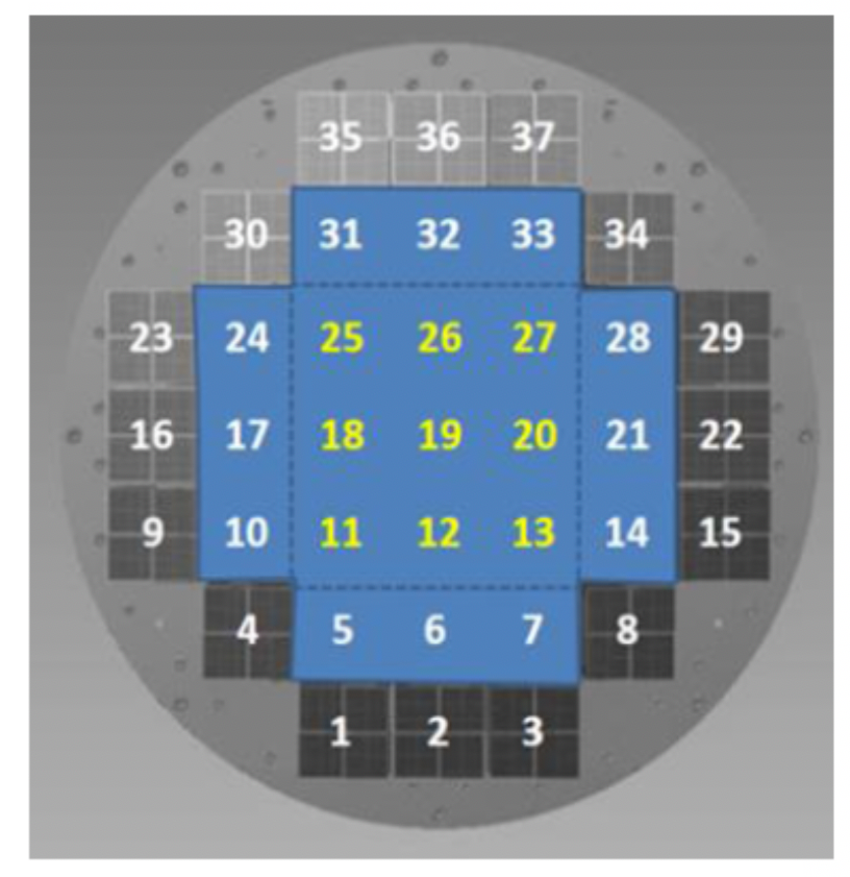
\includegraphics[height=7.9cm,angle=0,scale=1.0]{Figure/focal_plane.pdf}}
\caption{Scheme of the disposition of the PDMs on the focal surface. Numbers identify the PDM, the FoV common to UVscope is indicated with the dashed lines and with the yellow color of the PDMs.}
\label{fig:camera}
\end{figure}

Each PDM is composed of 8$\times$8 side-by-side Silicon photomultipliers (SiPMs). The front-end electronics (FEE) is composed by two application specific integrated circuits (ASIC), CITIROC. This represent an innovative solution to acquire the SiPM output signals  being based on a custom peak-detector operation mode rather than the usually adopted sampling technique \citep{Sottile2016}. 
Two separate electronics chains allow for high- and low-gain (HG and LG). The outputs of all  channels is read out by multiplexing, in parallel, the analog buffers of the HG and LG chains in two external analog-to-digital converter (ADC).
The signal is amplified by the programmable preamplifiers one relative to each chain and then shaped with a constant
shaping time of 37.5 ns and, in peak detector mode, the maximum of the shaped pulse height is registered. 

This FEE-FPGA manages the the generation of local trigger, a topological one, activated when a given number of contiguous pixels within a PDM presents a signal above a given photo-electron threshold \citep{Sottile2016}.
The back-end electronics (BEE) is the main elaboration unit of the camera which controls and manages the overall system, including data, and all ancillaries used to perform operations as
the camera thermal regulation, the voltage distribution management and the time events stamping.
The BEE also provides the functions necessary to process and transmit the event data as obtained by the FEE to an external data acquisition workstation responsible for receiving and storing the data packets \citep{Sottile2016}.
In order to protect the camera sensors from the external
atmospheric environment, an optical-UV transparent poly methyl methacrylate (PMMA)  window 
is mounted onto the focal surface support structure covering all the PDMs.
This window is modeled with the same radius of curvature of the focal surface \citep{Catalano2018}.
The ASTRI SST-2M camera is also equipped  with a light-tight lid to prevents accidental sunlight 
exposure of the focal surface detectors.
The camera is thermally controlled to keep the working temperature on the focal plane within the range 13-17$^\circ$C
for maintaining a good gain stability, considering that the gain variation with the temperature are of the order of 1 ADC per C$^\circ$ \citep{Impiombato2015}.


ASTRI-Horn read out electronics is AC-coupled to the detector output, and any slow varying signal is  blocked.
The camera is then blind to the diffuse night sky background (NSB) or to the light from stars in the FoV.   However, considering that sky photons actually arrive with a random Poisson time distribution, the fluctuations generated in the electronic signal are detected as noise. ASTRI-Horn  background is then characterised by signals distributed around an constant average value (pedestal) with fluctuations whose standard deviation is due both to the intrinsic electronic noise and to the NSB flux.  The total standard deviation of the background in the camera is obtained by the following formula:

\begin{equation}
\sigma^2=\sigma^2_{dk}+\sigma^2_{sky}
\end{equation}

\noindent
where $\sigma_{dk}$ is the intrinsic standard deviation of the electronics plus the detector noise observed in complete dark condition, as with the lid closed, and $\sigma_{sky}$ is the standard deviation induced by the  NSB  which is directly proportional to the photon flux.

